\documentclass[12pt,oneside]{report}

\usepackage[left=1.5in,right=1in,top=1.5in,bottom=1in,includehead]{geometry}
\usepackage{newtxtext}
\usepackage{newtxmath}
\usepackage{setspace}
\usepackage{graphicx}
\usepackage{booktabs}
\usepackage{longtable}
\usepackage{array}
\usepackage{tabularx}
\usepackage{multirow}
\usepackage{amsmath}
\usepackage{caption}
\usepackage{float}
\usepackage{fancyhdr}
\usepackage[hidelinks]{hyperref}
\usepackage{titlesec}
\usepackage{enumitem}
\usepackage{url}
\usepackage{tikz}
\usepackage{pgfplots}
\usetikzlibrary{arrows.meta,positioning,shapes.geometric,fit,calc}
\pgfplotsset{compat=1.18}

\setstretch{2.0}
\setlength{\parindent}{0.5in}
\setlength{\parskip}{0pt}
\setlength{\headheight}{15pt}
\captionsetup{font=small}
\captionsetup{skip=4pt}
\AtBeginEnvironment{figure}{\singlespacing}
\AtBeginEnvironment{table}{\singlespacing}

\pagestyle{fancy}
\fancyhf{}
\fancyhead[R]{\thepage}
\renewcommand{\headrulewidth}{0pt}

\titleformat{\chapter}[hang]
  {\normalfont\bfseries\Large}
  {\thechapter.}
  {0.6em}
  {}
\titlespacing*{\chapter}{0pt}{0pt}{12pt}

\newcommand{\AltText}[1]{\par\small\textit{Alternative text: #1}\normalsize}
\newcommand{\FormulaAlt}[1]{\par\small\textit{Alternative text for equation: #1}\normalsize}
\newcommand{\ReportTitle}{HYBRID VIDEO WATERMARKING FOR OTT PIRACY PREVENTION USING CONTENT-AWARE PLACEMENT, FORENSIC TRACEABILITY, AND ROBUST DETECTION}
\newcommand{\StudentName}{SubhaSai DurgaVenkata Vinnakota}
\newcommand{\DegreeName}{MASTER OF SCIENCE}
\newcommand{\MajorName}{Computer Science}
\newcommand{\DepartmentName}{Computer Science}
\newcommand{\TermName}{SPRING}
\newcommand{\TermYear}{2026}
\newcommand{\CommitteeChair}{Dr. Bang Tran S}
\newcommand{\SecondReader}{Dr. Ying Jin}
\newcommand{\GraduateCoordinator}{Dr. Haiquan Chen}
\newcommand{\PlaceholderFigure}[2]{
\begin{figure}[htbp]
\centering
\fbox{\parbox{0.82\textwidth}{\centering
\vspace{1.4in}
Placeholder for #1

Replace this placeholder with the exported diagram, screenshot, or chart before final submission.
\vspace{1.4in}}}
\caption{#1}
\AltText{#2}
\end{figure}
}

\begin{document}
\pagenumbering{arabic}

\begin{titlepage}
\thispagestyle{empty}
\begin{center}
\vspace*{0.4in}
{\Large\bfseries \ReportTitle\par}
\vspace{1.4in}
A Project\par
\vspace{1.2in}
\begin{spacing}{1.0}
Presented to the faculty of the Department of \DepartmentName\par
California State University, Sacramento\par
\end{spacing}
\vspace{1.2in}
\begin{spacing}{1.0}
Submitted in partial satisfaction of\par
the requirements for the degree of\par
\end{spacing}
\vspace{0.6in}
{\large \DegreeName\par}
\vspace{0.5in}
in\par
\vspace{0.3in}
{\large \MajorName\par}
\vspace{1.1in}
by\par
\vspace{0.5in}
{\large \StudentName\par}
\vfill
\TermName\par
\TermYear
\end{center}
\end{titlepage}

\clearpage
\thispagestyle{empty}
\begin{center}
\ReportTitle
\vspace{1.0in}

A Project
\vspace{1.0in}

by
\vspace{1.0in}

\StudentName
\end{center}
\vspace{1.2in}
\noindent
Approved by:

\vspace{1.0in}
\noindent
\rule{4.5in}{0.4pt}\\
{\CommitteeChair, Committee Chair}

\vspace{0.5in}
\noindent
\hspace*{0.1in}Date

\vspace{1.0in}
\noindent
\rule{4.5in}{0.4pt}\\
{\SecondReader, Second Reader}

\vspace{1.0in}
\noindent
\hspace*{0.1in}Date

\clearpage
\thispagestyle{empty}

\vspace*{2.0in}
\noindent
Student: \StudentName

\vspace{0.8in}
\noindent
I certify that this student has met the requirements for format contained in the University format manual, and this project is suitable for electronic submission to the library and credit is to be awarded for the project.

\vspace{1.0in}
\noindent
\rule{3.7in}{0.4pt}\hfill Date\\
\GraduateCoordinator, Graduate Coordinator

\vspace{0.8in}
\noindent
Department of \DepartmentName

\clearpage
\thispagestyle{empty}
\begin{center}
Abstract

\vspace{0.3in}
of

\vspace{0.3in}
\ReportTitle

\vspace{0.6in}
by

\vspace{0.3in}
\StudentName
\end{center}

\vspace{0.6in}
\noindent\textbf{Statement of Problem}

This project studies how to watermark video in a way that is practical for over-the-top streaming platforms. The main goal is to place a visible watermark where it is less distracting while still keeping it recoverable after common distortions such as re-encoding, blur, crop, grayscale conversion, frame-rate reduction, and resize. A second goal is traceability, so that a leaked copy can still be tied back to a user or session. To address both needs, the project combines visible watermarking, invisible payload embedding, detection, attack testing, and a user-facing application in one workflow.

\vspace{0.3in}
\noindent\textbf{Sources of Data}

The implemented system uses Laplacian-based complexity, semantic saliency from pretrained models, temporal smoothing, optional optical flow, visible text rendering, discrete cosine transform payload embedding, and a neural watermarking branch. It also stores frame-level placement metadata in a \texttt{positions.json} file so that detection can use both local search and a global fallback when the watermark shifts after attack. The broader project workflow draws on a standardized 150-clip training corpus for model development and a separate 26-clip HD benchmark for visible robustness evaluation. In that benchmark, the visible channel achieved 94.6\% mean detection at a normalized cross-correlation threshold of 0.40, while later local batch evaluation showed that the DCT and neural channels can provide useful supporting forensic information.

\vspace{0.3in}
\noindent\textbf{Conclusions Reached}

The main conclusion is that content-aware visible watermarking is the strongest and most mature part of the system. The DCT and neural branches make the design more complete and more useful for forensic tracing, but they still involve stronger quality-versus-robustness tradeoffs. Overall, the project delivers a full workflow for watermark generation, manual adjustment, detection, attack testing, and traceability in a form that is technically credible, practical to demonstrate, and well suited to a master's final project.

\vspace{0.8in}
\noindent\hfill\rule{2.8in}{0.4pt}

\noindent\hfill\CommitteeChair, Committee Chair

\vspace{0.6in}
\noindent\hfill\rule{2.0in}{0.4pt}

\noindent\hfill Date

\clearpage
\chapter*{Acknowledgements}
\addcontentsline{toc}{chapter}{Acknowledgements}
I would like to express my sincere gratitude to my project advisor for the guidance, patience, and insights that shaped every stage of this work. The regular feedback sessions were essential in refining both the software and this written report.

I am grateful to the faculty of the Department of Computer Science at California State University, Sacramento, whose coursework in software engineering, data science, and related areas provided an important foundation for this project. I also thank the second reader and committee members for suggestions that improved the clarity of the manuscript.

Special thanks go to the open-source communities behind OpenCV, PyTorch, Streamlit, FastAPI, and FFmpeg, whose freely available tools made this project possible. Finally, I thank my family and friends for their encouragement and support throughout my graduate studies.

\clearpage
\begingroup
\singlespacing
\tableofcontents
\endgroup
\clearpage
\begingroup
\singlespacing
\listoffigures
\endgroup

\clearpage
\chapter{INTRODUCTION}
\section{Purpose}
This project was carried out to build and evaluate a practical video watermarking system for piracy deterrence and traceability in over-the-top streaming settings. The work sits between two common extremes. On one side are simple visible overlays that are easy to add but often distract viewers and can be removed by basic editing. On the other side are more advanced invisible watermarking ideas that are promising in theory but harder to reproduce, explain, and connect to a usable application. The purpose of this project was to bring those worlds together in a single system that could be tested, demonstrated, and discussed clearly.

The main idea behind the project is straightforward: watermarking should not be treated as a single drawing step. A useful system has to decide where the watermark should go, how strong it should be, how it should be recovered later, and how the output can be traced back to a specific viewer when needed. Those choices affect each other. A watermark that looks better may be harder to recover. A watermark that is easier to detect may be more distracting. The project therefore approaches watermarking as a balanced engineering problem rather than as a search for one perfect algorithm.

\section{Problem}
Video piracy is still a serious problem for streaming platforms because a video can be screen-recorded, re-encoded, cropped, reposted, and shared widely with very little effort. Visible watermarks are still widely used because they are easy to understand and can directly show ownership or a user identifier. Their weakness is that they can become annoying if they cover a face, text, or another important part of the frame. Invisible watermarks help with forensic tracing, but they raise different problems around quality, robustness, and implementation effort. The core problem in this project is therefore the following: \textit{how can a video watermarking system place a visible watermark in a less distracting area, add invisible support when needed, and still detect the watermark reliably after common attacks, all within a usable software application?}

This problem breaks into four practical questions. First, the system must solve the \textbf{placement problem}: where should the watermark go so that it does not distract the viewer too much? Second, it must solve the \textbf{stability problem}: how can it avoid jitter from one frame to the next? Third, it must solve the \textbf{detection problem}: how can it still find the watermark after crop, compression, blur, or resize? Fourth, it must solve the \textbf{traceability problem}: how can the output be tied to a specific user, session, or device? These questions guide the rest of the report.

\section{Project Scope}
The scope of the project spans both research and software engineering. On the research side, it covers visible placement, DCT watermarking, neural watermarking, error correction, and robust detection. On the engineering side, it includes a Streamlit interface, attack testing, manual adjustment, a FastAPI service, and HLS scaffolding. At the same time, the project stays within clear limits. It does not claim to be a commercial forensic watermarking product, and it does not claim that its invisible channels outperform specialized industrial systems. Its contribution is a solid, well-documented academic prototype that can be tested and extended.

\section{Statement of Collaboration}
This project was completed as an individual master's final year project under academic supervision. The work developed through repeated cycles of reading, prototyping, debugging, attack testing, UI refinement, and written review. Faculty feedback helped shape the project goals and the final report, while open-source libraries and pretrained models provided the technical building blocks used for saliency estimation, optical flow, and neural watermarking. Development also included AI-assisted iteration for coding support, debugging, and report refinement, while final design decisions, implementation integration, evaluation, and written responsibility remained with the author.

\section{Objectives}
The main objective was to build a system that could watermark videos in more than one way while still being understandable, testable, and easy to demonstrate. More specifically, the project aimed to support multiple placement modes, preserve temporal consistency, provide user-specific traceability, recover visible watermarks with strong detection logic, and expose the full workflow through an interactive application. Additional goals included U2-Net support, RAFT optical flow, HLS processing, a neural encoder-decoder branch, and baseline comparison scaffolding.

\begin{figure}[htbp]
\centering
\resizebox{0.96\textwidth}{!}{%
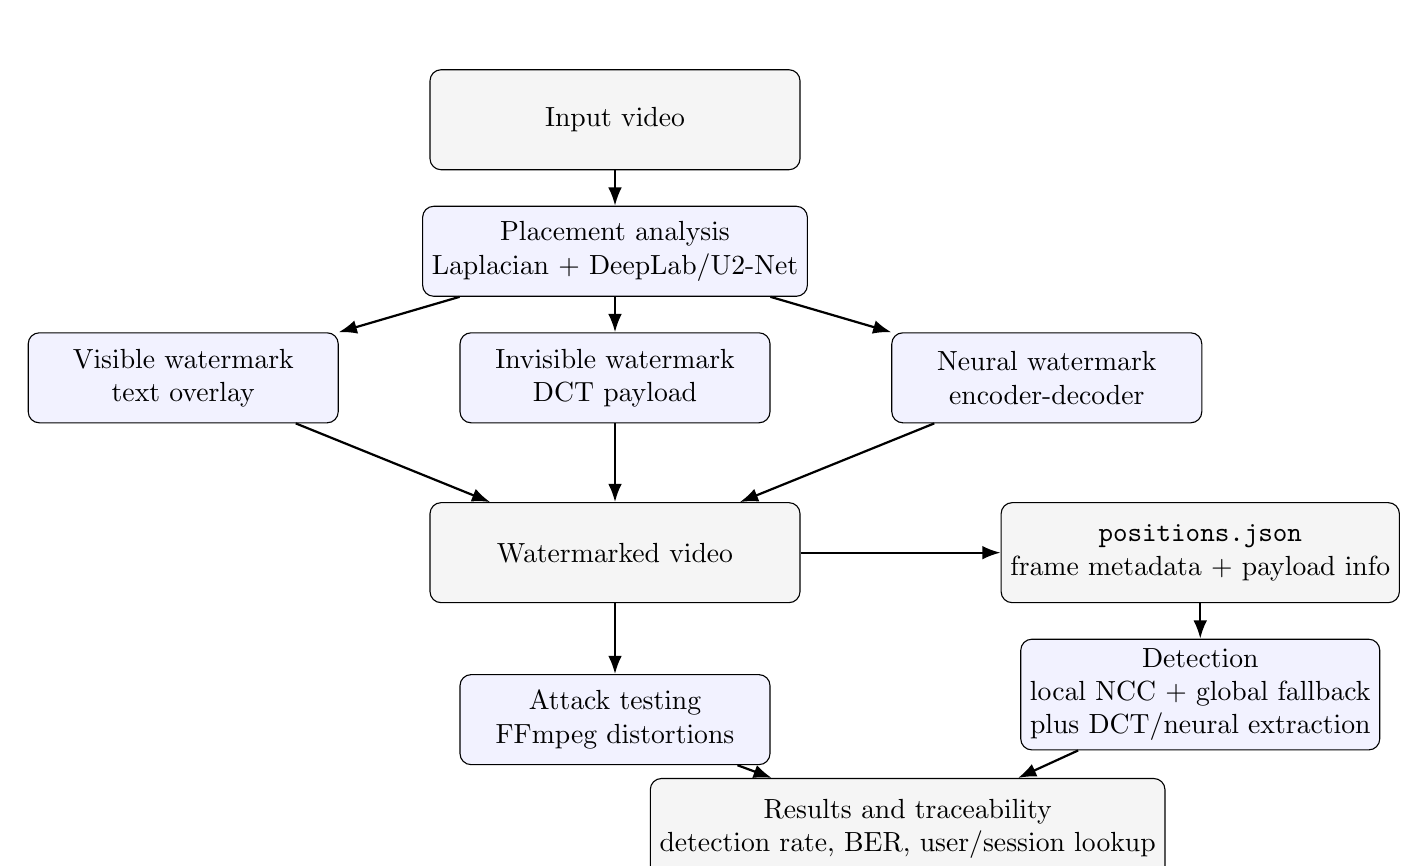
\begin{tikzpicture}[
node distance=0.45cm and 0.55cm,
box/.style={draw, rounded corners, align=center, minimum width=1.85in, minimum height=0.5in, fill=gray!8},
smallbox/.style={draw, rounded corners, align=center, minimum width=1.55in, minimum height=0.45in, fill=blue!5},
arrow/.style={-Latex, thick}
]
\node[box] (input) {Input video};
\node[smallbox, below=of input] (placement) {Placement analysis\\Laplacian + DeepLab/U2-Net};
\node[smallbox, below left=of placement, xshift=-0.2in] (visible) {Visible watermark\\text overlay};
\node[smallbox, below=of placement] (dct) {Invisible watermark\\DCT payload};
\node[smallbox, below right=of placement, xshift=0.2in] (neural) {Neural watermark\\encoder-decoder};
\node[box, below=1.0cm of dct] (output) {Watermarked video};
\node[box, right=1.0in of output] (meta) {\texttt{positions.json}\\frame metadata + payload info};
\node[smallbox, below=0.9cm of output] (attack) {Attack testing\\FFmpeg distortions};
\node[smallbox, below=of meta] (detect) {Detection\\local NCC + global fallback\\plus DCT/neural extraction};
\node[box, below=0.9cm of $(attack)!0.5!(detect)$] (trace) {Results and traceability\\detection rate, BER, user/session lookup};

\draw[arrow] (input) -- (placement);
\draw[arrow] (placement) -- (visible);
\draw[arrow] (placement) -- (dct);
\draw[arrow] (placement) -- (neural);
\draw[arrow] (visible) -- (output);
\draw[arrow] (dct) -- (output);
\draw[arrow] (neural) -- (output);
\draw[arrow] (output) -- (attack);
\draw[arrow] (output) -- (meta);
\draw[arrow] (attack) -- (trace);
\draw[arrow] (meta) -- (detect);
\draw[arrow] (detect) -- (trace);
\end{tikzpicture}
}
\caption{Overall project architecture for the hybrid visible, DCT, and neural watermarking pipeline}
\AltText{A system diagram showing an input video feeding a placement analysis stage, which then branches into visible text rendering, DCT embedding, and neural watermarking. The watermarked output is stored with a positions file and later used by attack testing and detection to produce robustness and traceability results.}
\end{figure}

\section{Research Questions}
The project was guided by four main questions: can adaptive placement make a visible watermark less distracting than fixed placement, does global fallback materially improve recovery after crop and resize attacks, can the system support practical traceability through visible and invisible payloads, and how far can DCT and neural watermarking be pushed before quality and robustness begin to conflict too strongly? These questions shape the rest of the report.

\section{Report Organization}
The remainder of this report is organized as follows. Chapter 2 reviews the technical background of digital watermarking, content-aware placement, forensic payload encoding, optical flow stabilization, and neural watermarking. Chapter 3 presents the design methodology, including system architecture, mathematical formulation, and module-level integration. Chapter 4 describes implementation details and experimental results, including benchmark metrics and discussion of quality-robustness tradeoffs. Chapter 5 concludes the project and identifies limitations and realistic future extensions.

\clearpage
\chapter{BACKGROUND OF THE STUDY}
\section{Digital Watermarking in Multimedia Systems}
Digital watermarking is broadly concerned with embedding identifying information into media such that the media remains usable while the identifying information remains recoverable or at least detectable. In the context of video, the design space becomes more complex than in still images because temporal consistency matters. A watermark that moves erratically between adjacent frames may technically exist, yet still fail from a user-experience perspective because the overlay draws attention to itself. Similarly, a watermark that is recoverable from a single frame under laboratory conditions may fail when an attacker crops the frame, reduces the resolution, changes the frame rate, or re-encodes the video using aggressive compression settings. This means that practical video watermarking sits at the intersection of image processing, signal processing, human perception, and systems integration.

Watermarking schemes are often classified as visible or invisible. Visible watermarks are explicitly presented to the viewer, typically as text, logos, or translucent overlays. Their strengths include simplicity, immediate deterrence value, and straightforward visual verification. Their weaknesses include possible obstruction of important content and susceptibility to removal through inpainting, crop, or re-recording. Invisible watermarks hide the payload within the signal itself. Their strengths include lower perceptual impact and stronger forensic utility. Their weaknesses include sensitivity to attacks, the need for more specialized recovery logic, and the possibility of difficult robustness-visibility tradeoffs. In practice, many real-world systems benefit from hybrid strategies in which a visible channel provides deterrence while an invisible channel provides redundancy and forensic support.

\section{Visible Watermark Placement and Perceptual Considerations}
Visible watermarking is not only a rendering task but also a placement task. If a watermark lies directly across a speaker's face, over subtitle text, or in the center of a high-motion action scene, viewers experience it as an obstruction rather than as a low-level protective feature. The problem of \textit{where} to place the watermark is therefore closely related to visual attention and saliency. Early approaches frequently relied on heuristics such as placing the overlay in a corner or over smooth areas. Such methods are appealing because they are computationally cheap, but they struggle when a corner contains meaningful content or when the visual structure of the frame changes over time.

Structural measures such as edge strength or local variance provide one family of placement signals. A Laplacian-based complexity map is particularly attractive because it is easy to compute and intuitively interpretable: smooth areas such as sky, wall, or road tend to yield lower magnitude responses than highly textured regions. When the watermark is semi-transparent, low-complexity regions often remain legible without dominating the frame. However, purely structural measures do not understand semantics. A face against a smooth background may have sharp boundaries but semantically still be the wrong place for a watermark. This limitation motivates the use of semantic segmentation or saliency estimation as a second placement cue.

Research in saliency-guided placement suggests that the best visible watermark location is usually one that avoids dominant foreground objects and remains reasonably stable over time. Modern segmentation networks provide dense predictions that can distinguish people, vehicles, animals, and background surfaces. While they are not designed solely for watermark placement, they offer a useful approximation of semantic importance. By treating the background as relatively safe placement territory and the foreground as costly placement territory, a watermarking system can use segmentation output to supplement simpler structural cues.

\section{Template Matching and Normalized Cross-Correlation}
Visible watermark detection can be approached with machine learning, but template matching remains attractive when the watermark text, size, and approximate location are already known. Normalized cross-correlation is a standard method because it scores the similarity between a template and a search region while reducing sensitivity to global brightness changes. Lewis's work on fast normalized cross-correlation established a strong basis for practical template-based image matching, and the technique remains widely used because of its simplicity and interpretability. In the context of this project, normalized cross-correlation offers a pragmatic solution that fits well with visible text overlays and saved placement metadata.

Nevertheless, plain template matching is rarely enough by itself. If the template is searched at only one size, even modest resizing will reduce detection performance. If the search region is limited strictly to the originally saved coordinates, crop and geometry changes may shift the watermark outside the expected region. For these reasons, the project adopts a multi-scale template search over both a local region of interest and, when the local score fails, a downscaled global fallback search. This combination keeps normal cases fast while preserving robustness in difficult cases.

\section{Discrete Cosine Transform Watermarking}
Transform-domain watermarking is a classic approach in which information is embedded not directly into pixel intensities but into transformed coefficients that represent frequency content. The discrete cosine transform is especially common because of its close relationship to JPEG and other compression schemes. Mid-frequency coefficients are often preferred for watermarking because low-frequency coefficients strongly influence visible appearance while high-frequency coefficients are more likely to be suppressed by compression or filtering. Embedding in a carefully chosen set of mid-frequency coefficients can therefore provide a workable compromise between invisibility and recoverability.

The DCT branch in this project follows that logic. It operates on luminance, uses 8x8 blocks, and embeds bits in selected mid-band coefficients. This aligns well with prior signal-processing intuition: changes in the luminance channel can be spread across the transform domain, and a block-based approach remains computationally manageable in video processing. Yet, as with all watermarking techniques, DCT embedding alone is not enough. If the payload is short and errors occur under attack, the receiver needs some mechanism to reconstruct the intended information. This is where error correction becomes important.

\section{Error Correction and Encrypted Payloads}
For forensic traceability, merely embedding bytes is not sufficient when distortion can flip bits or corrupt whole symbol groups. Reed-Solomon coding is a natural fit because it corrects symbol errors and burst-like corruption effectively. In multimedia watermarking, it is frequently used to protect short identifiers, session markers, or authentication data. By encoding the payload before embedding, the decoder can tolerate some corruption without losing the overall message. This is particularly important in a project setting where invisible payload channels are expected to coexist with visible overlays and post-processing attacks.

AES-GCM serves a different purpose. Rather than improving raw robustness, it protects confidentiality and integrity when payload contents should not appear in plaintext. In a forensic watermarking workflow, a platform may wish to embed a compact session token or user reference that should only be recoverable in controlled conditions. Combining Reed-Solomon with optional AES-GCM therefore supports both error resilience and data protection. In this project, the cryptographic and error-correction layers are treated as optional but important deployment-oriented features that bring the implementation closer to realistic streaming use cases.

\section{Optical Flow and Temporal Consistency}
Temporal consistency is crucial in video watermark placement because human observers are highly sensitive to jitter. If a watermark is recalculated independently on every frame, even small changes in scene content can make the chosen position oscillate between nearby regions. Such oscillation makes the watermark more noticeable. Exponential moving average smoothing is a simple and effective first step because it biases the current position toward the previous one. However, EMA alone does not exploit actual scene motion. If the camera pans or the background moves, the preferred region itself may shift in ways that EMA can only partially track.

Optical flow addresses this by estimating apparent motion between adjacent frames. Farneback's dense flow method remains popular because it is relatively lightweight and available in OpenCV. RAFT represents a more modern deep-learning approach with higher computational cost but often stronger accuracy. In the watermarking context, optical flow can be used to warp the previous frame's placement guide map into the current frame's coordinates. The current frame then blends its own guide map with the warped historical estimate, encouraging the watermark to stay attached to semantically stable background regions rather than jittering independently.

\section{Deep Learning for Saliency and Neural Watermarking}
Deep learning contributes to this project in two distinct ways. The first is semantic saliency for visible watermark placement. DeepLabV3 and U2-Net are not watermarking models in the narrow sense, but they provide information about what parts of the scene are likely to be foreground objects or visually important regions. This information improves placement quality because the watermark can preferentially avoid those regions. The second contribution is the neural watermarking branch itself, where an encoder-decoder architecture attempts to embed and recover a hidden bitstring directly from the visual signal.

Neural watermarking is attractive because it can potentially learn robust, distributed signal patterns rather than relying only on hand-designed frequency coefficients. However, it is also difficult. The network must preserve appearance, survive attacks, and still recover the payload. Even when training succeeds on images, transferring the method to full videos introduces additional complications such as frame resizing, temporal consistency, and perceptual quality. For that reason, the neural branch in this project is valuable both as a functional prototype and as a demonstration of the tradeoffs involved in machine-learned watermarking systems.

\section{OTT Piracy Prevention and Forensic Watermarking}
From an application standpoint, over-the-top piracy prevention is one of the strongest real-world motivations for watermarking. In a streaming service, the platform often needs not only to signal ownership but also to identify which subscriber copy or which distribution session leaked content. This leads to the concept of forensic watermarking, where each distributed copy may contain individualized identifiers. A forensic watermark does not need to stop every leak preemptively; its value lies in supporting post hoc attribution and deterrence. If users know that their copy can be linked back to their account, some forms of redistribution may be discouraged.

The project adopts this perspective by supporting both direct identifiers and hashed identifiers in the visible watermark text. It also adds invisible payload mechanisms so that visible and invisible channels can reinforce each other. This hybrid approach is well aligned with OTT use cases, where different deployment environments may prioritize deterrence, aesthetics, traceability, or all three at once.

\section{Research Gap and Project Positioning}
The literature and tooling landscape suggest a gap that is well suited to a master's project. There are many components available in isolation: saliency estimation, transform-domain watermarking, neural image watermarking, optical flow, cryptographic payload protection, and web application frameworks. What is less common in student-scale academic projects is an integrated pipeline that joins these pieces into a usable, inspectable, and benchmarked system. This project positions itself in that gap. Its contribution is not the invention of a wholly new watermarking primitive. Rather, it is the design and evaluation of a coherent hybrid watermarking system that combines content-aware placement, robust visible detection, forensic payload handling, and interactive tooling in a reproducible framework.

\clearpage
\chapter{METHODOLOGY AND SYSTEM DESIGN}
\section{Design Requirements}
The methodology began from a concrete set of system requirements. The watermark needed to be visible enough to serve as a deterrent, but also sufficiently unobtrusive to preserve watchability. The system needed to save enough metadata to support later detection. It needed to permit user-specific or session-specific identifiers so that the output could serve forensic goals. The detection path needed to tolerate ordinary distribution artifacts such as compression and scaling. The implementation also needed to remain accessible to non-expert users, which motivated the inclusion of an interactive application rather than only command-line scripts.

These requirements produced the architecture shown conceptually in the workflow documentation. A frame-level placement pipeline generates the visible overlay coordinates; an embedding pipeline renders the visible and optional invisible watermarks; a metadata layer stores per-frame positions and payload information; and a detection layer consumes both the attacked video and the metadata file. The major methodological decision was to preserve this metadata explicitly rather than rely only on blind detection. For a visible watermarking system intended for operational use, keeping a synchronized placement record is a reasonable engineering choice that greatly simplifies detection and analysis.

\section{System Architecture}
The system can be understood as six cooperating layers: interface, placement, embedding, metadata, detection, and evaluation. The Streamlit interface manages user interaction and orchestrates the pipeline. The placement layer computes one or more guidance maps and chooses the least intrusive region. The embedding layer renders visible text and optionally inserts invisible DCT or neural content. The metadata layer serializes the placement and payload context into \texttt{positions.json}. The detection layer reconstructs the watermark template and searches for it using normalized cross-correlation. Finally, the evaluation layer applies attacks and aggregates recovery statistics.

In software terms, \texttt{src/app\_watermark\_ui.py} controls the user workflow, \texttt{src/video\_watermark\_demo.py} handles most watermarking logic, \texttt{src/detect\_watermark.py} handles visible detection, \texttt{src/dct\_watermark.py} handles transform-domain payloads, and the neural branch is grouped under \texttt{src/neural\_watermark/}. This modular structure made the project easier to test and extend.

\section{Visible Placement Method}
\subsection{Laplacian Complexity Map}
The first placement signal is structural complexity. For each frame, the system converts the image to grayscale, applies a Gaussian blur, computes a Laplacian response, takes the absolute value, and normalizes the result to the interval $[0,1]$. The intent is not to classify objects but to approximate how visually busy each region is. Smooth regions such as sky, walls, or roads tend to produce lower values than textured foliage, text, or facial details. The complexity map is therefore an economical proxy for perceptual unobtrusiveness.

Mathematically, if $I$ denotes the grayscale frame and $B_{\sigma}(I)$ denotes Gaussian smoothing with standard deviation $\sigma$, the structural map $L$ can be expressed as
\begin{equation}
L = \mathrm{Normalize}\left(\left|\nabla^2 B_{\sigma}(I)\right|\right).
\end{equation}
\FormulaAlt{The Laplacian complexity equation states that the system computes a blurred grayscale image, applies the Laplacian operator, takes the magnitude, and normalizes the result so that low values correspond to smoother regions.}

This signal alone already provides a useful baseline because many objectionable placements occur on high-frequency content where a watermark is visually disruptive. However, complexity alone can still choose semantically wrong regions. For that reason, the system augments it with semantic saliency.

\subsection{Semantic Saliency Map}
The semantic branch uses pretrained segmentation output to estimate which pixels are likely to belong to foreground objects versus background. In the DeepLab configuration, the model predicts a dense label field, and the implementation interprets background-like predictions as more suitable placement territory. The project also includes U2-Net support as an alternate saliency model. The semantic map, denoted $D$, is again normalized to $[0,1]$, with lower values indicating more acceptable regions for watermark placement.

This choice reflects a practical observation: even when a visually smooth region exists on a person, vehicle, or another salient object, it is often a poor location for a visible watermark because the human observer is already attending to that object. A background-aware semantic map therefore corrects some of the mistakes made by purely structural placement logic.

\subsection{Hybrid Fusion}
The project's default strategy is to fuse the structural and semantic maps into a single guide map $G$. If $L$ denotes the Laplacian complexity map and $D$ denotes the semantic saliency map, then the hybrid guide map is
\begin{equation}
G = (1 - w_D)L + w_D D,
\end{equation}
where $w_D$ is the weight given to the semantic branch. In the implementation and benchmark narrative, the default value is $w_D = 0.6$.
\FormulaAlt{The hybrid fusion equation states that the final placement cost map is a weighted average of the Laplacian structural map and the semantic saliency map, with the semantic map receiving weight 0.6 by default.}

This design choice is intentionally conservative. A purely semantic approach can be unstable or overly coarse, while a purely structural approach ignores meaning. The weighted combination lets the system benefit from both. Normalization keeps the two maps on comparable scales before fusion, and the final map is again normalized to preserve interpretability.

\subsection{Sliding-Window Selection and Edge Preference}
Once the guide map has been produced, the system defines a candidate watermark box based on text size, font scale, and padding, then slides that box across the guide map using a stride of 32 pixels. For each candidate top-left coordinate $(x,y)$, the system computes the mean value inside the window. The coordinate with the lowest average cost is selected, subject to optional edge constraints.

If $W_{x,y}$ denotes the window at position $(x,y)$, then the score used for candidate comparison is
\begin{equation}
S(x,y) = \frac{1}{|W_{x,y}|}\sum_{(i,j)\in W_{x,y}} G(i,j).
\end{equation}
\FormulaAlt{The sliding-window scoring equation states that each candidate watermark position is evaluated by averaging the hybrid placement cost map over the watermark-sized window, and the system chooses the position with the lowest average value.}

The project also introduces an edge-biased mode, where only windows whose centers fall within an outer edge band are considered. The default margin in the documented pipeline is approximately 12\% of the frame dimensions. This decision arises from a practical tradeoff. A corner or edge watermark is often less intrusive and sometimes harder to remove without visibly cropping the video. However, edge placement also risks damage under aggressive crop attacks. The benchmark results therefore evaluate not only ordinary detection but also the behavior of the system under cropping.

\subsection{Temporal Smoothing and Optical Flow}
If the system chooses a candidate position independently on every frame, small fluctuations in saliency values can produce visible jitter. To reduce this effect, the project applies exponential moving average smoothing to the chosen coordinates. If $(x_{\mathrm{cand}}, y_{\mathrm{cand}})$ is the current candidate and $(x_{t-1}, y_{t-1})$ is the previous smoothed position, the new position is
\begin{equation}
(x_t, y_t) = \alpha (x_{t-1}, y_{t-1}) + (1-\alpha)(x_{\mathrm{cand}}, y_{\mathrm{cand}}),
\end{equation}
with $\alpha = 0.8$ in the documented setup.
\FormulaAlt{The temporal smoothing equation states that the new watermark location is a weighted blend of the previous smoothed location and the current candidate location, with 80 percent weight on the previous location.}

EMA is supplemented by a maximum-jump rule so that genuine scene changes are not artificially over-smoothed. Optional optical flow further stabilizes the placement process by warping the previous frame's guide map into the current frame. In effect, this gives the system a motion-aware memory of where low-cost placement regions are moving. Farneback flow offers a classical dense-motion estimate; RAFT offers a deep-learning alternative. The project supports both because computational cost and accuracy requirements vary by deployment scenario.

\begin{figure}[htbp]
\centering
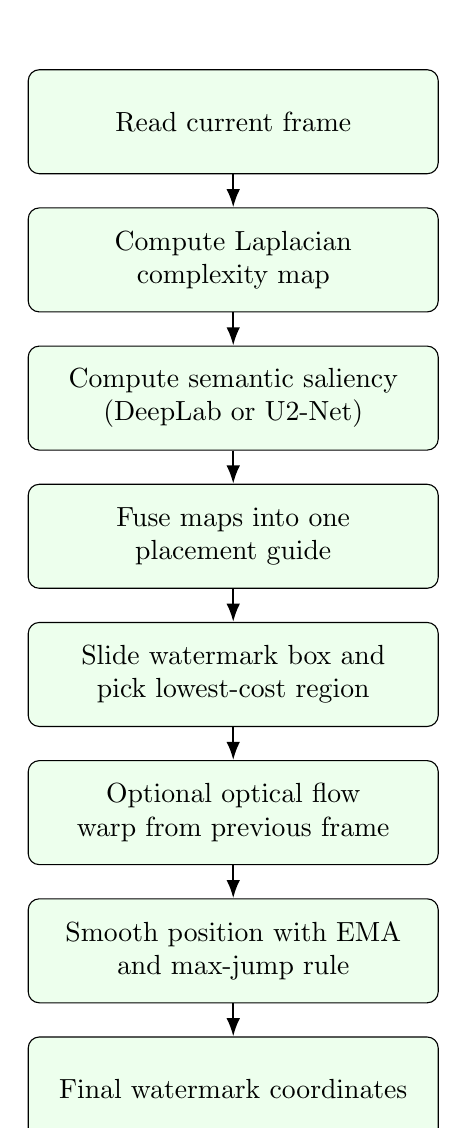
\begin{tikzpicture}[
node distance=0.42cm and 0.55cm,
flowstep/.style={draw, rounded corners, align=center, minimum width=2.05in, minimum height=0.52in, fill=green!7},
arrow/.style={-Latex, thick}
]
\node[flowstep] (frame) {Read current frame};
\node[flowstep, below=of frame] (lap) {Compute Laplacian\\complexity map};
\node[flowstep, below=of lap] (sal) {Compute semantic saliency\\(DeepLab or U2-Net)};
\node[flowstep, below=of sal] (fuse) {Fuse maps into one\\placement guide};
\node[flowstep, below=of fuse] (slide) {Slide watermark box and\\pick lowest-cost region};
\node[flowstep, below=of slide] (flow) {Optional optical flow\\warp from previous frame};
\node[flowstep, below=of flow] (ema) {Smooth position with EMA\\and max-jump rule};
\node[flowstep, below=of ema] (final) {Final watermark coordinates};
\draw[arrow] (frame) -- (lap);
\draw[arrow] (lap) -- (sal);
\draw[arrow] (sal) -- (fuse);
\draw[arrow] (fuse) -- (slide);
\draw[arrow] (slide) -- (flow);
\draw[arrow] (flow) -- (ema);
\draw[arrow] (ema) -- (final);
\end{tikzpicture}
\caption{Placement pipeline from frame input to smoothed watermark coordinates}
\AltText{A step-by-step flowchart showing the visible placement pipeline: reading a frame, building a Laplacian map, computing semantic saliency, fusing the maps, choosing a low-cost window, optionally warping the guide with optical flow, smoothing the result over time, and producing the final watermark position.}
\end{figure}

\section{Visible Rendering}
Once the position is selected, the visible watermark is rendered using OpenCV's text rendering and alpha blending. The font scale is adjusted relative to frame width so that the watermark remains legible across common resolutions. The implementation stores the text, font scale, thickness, box dimensions, opacity, and frame-wise coordinates in the metadata file. This record is important because it makes later detection and manual re-export deterministic. Without this saved context, detection would need to infer template size and expected location blindly, which would substantially complicate the pipeline.

The rendering itself is intentionally simple. A copy of the frame is created, text is drawn on the copy, and the copy is blended back into the original frame with user-selected opacity. This simplicity is a strength. It makes the visible channel easy to explain, easy to reproduce, and easy to benchmark. In a graduate project where the more advanced components already introduce uncertainty, the visible rendering path provides a reliable anchor for the whole system.

\section{DCT Invisible Payload Channel}
\subsection{Payload Construction}
The DCT branch embeds forensic payload bytes into luminance coefficients. Payload construction begins either from a user-visible identifier or from a more structured traceability record. The system supports direct identifiers and hashed forms, while the cryptographic payload utilities support optional AES-GCM encryption and Reed-Solomon coding. A length prefix is included so that extraction can determine where the payload ends. This is methodologically important because a short and explicit payload structure is easier to recover robustly than an open-ended byte stream.

\subsection{Block-Domain Embedding}
The DCT embedder processes the region of interest in $8 \times 8$ blocks. For each block, a discrete cosine transform is computed, selected mid-frequency coefficients are modified according to the payload bit sequence, and the inverse transform reconstructs the marked block. Embedding in the luminance channel is consistent with common compression-domain intuition, and using a localized region of interest keeps the invisible payload spatially separated from the visible text overlay.

Conceptually, if $C_{u,v}$ denotes the DCT coefficient at frequency index $(u,v)$ and $\Delta$ denotes an embedding perturbation determined by the bit value, the coefficient update follows the general pattern
\begin{equation}
\hat{C}_{u,v} = C_{u,v} + \Delta(b),
\end{equation}
where $b \in \{0,1\}$ denotes the embedded bit and the exact perturbation rule depends on the implementation's coefficient manipulation strategy.
\FormulaAlt{The DCT embedding equation states that selected transform coefficients are perturbed by an amount determined by the payload bit, after which the inverse transform reconstructs the watermarked block.}

The ROI is selected near but not directly overlapping the visible watermark. This separation reduces the risk that the visible overlay itself corrupts invisible payload recovery. Edge feathering is also used at ROI boundaries to minimize visible seams.

\subsection{Recovery and Interpretation}
During extraction, the DCT branch reprocesses the corresponding ROI, re-estimates bits from the selected coefficients, reconstructs the payload byte stream, and applies Reed-Solomon decoding when enabled. The project evaluates both extraction success and bit error rate, since a binary ``extracted'' label alone can hide significant corruption. The local batch evaluation summaries show that DCT extraction is not uniformly reliable under all attacks, but it still provides a useful invisible redundancy channel within the overall hybrid design.

\section{Neural Watermarking Branch}
\subsection{Encoder-Decoder Design}
The neural watermarking branch uses a U-Net-like encoder-decoder architecture. Payload bits are expanded spatially and concatenated with the cover image channels so that the encoder can condition its perturbation on the desired bit sequence. The encoder predicts a residual watermark pattern, or \textit{delta}, which is scaled and added to the input image. A decoder network then attempts to recover the payload bits from the watermarked image. This design follows a common residual-learning strategy in learned watermarking: instead of synthesizing the whole frame, the network learns only the perturbation that must be applied.

If $X$ denotes the cover frame, $p$ denotes the payload bit vector, and $E$ denotes the encoder network, then the watermarked output is
\begin{equation}
Y = \mathrm{clip}\left(X + \delta, 0, 1\right), \qquad \delta = E(X,p)\cdot \lambda,
\end{equation}
where $\lambda$ is a perturbation strength parameter referred to in the implementation as \texttt{delta\_scale}.
\FormulaAlt{The neural embedding equation states that the encoder produces a residual perturbation conditioned on the cover image and payload bits, scales it by the delta parameter, and adds it to the original image while clipping the final result to the valid range.}

The system later improved this inference path by upsampling only the learned delta back to the original frame resolution instead of replacing the full frame with an upscaled network output. This was an important engineering correction because direct replacement degraded fine texture and introduced color distortion.

\subsection{Training Strategy}
The training code supports a staged curriculum. Early phases emphasize learnability with reduced perceptual constraints, while later phases introduce stronger attack simulation and more balanced losses. The project includes a differentiable attack simulator for blur, additive noise, and resize down-up operations. This is useful because it encourages the encoder to produce a perturbation that remains decodable after likely distortions. An auxiliary delta decoder can also be used to provide additional gradient signal directly on the residual watermark pattern.

The loss function combines payload recovery terms with appearance preservation terms. At a high level, if $\mathcal{L}_{\mathrm{BCE}}$ denotes binary cross-entropy for payload bits, $\mathcal{L}_{\mathrm{MSE}}$ denotes appearance preservation error, and $\mathcal{L}_{\Delta}$ denotes an auxiliary residual decoding loss, the training objective can be written schematically as
\begin{equation}
\mathcal{L} = \mathcal{L}_{\mathrm{BCE}} + \beta \mathcal{L}_{\mathrm{MSE}} + \gamma \mathcal{L}_{\Delta}.
\end{equation}
\FormulaAlt{The neural training loss equation states that the total objective combines payload recovery error, appearance preservation error, and an optional residual-decoding loss, weighted by tuning parameters beta and gamma.}

Even with this design, the neural channel remains the most difficult component of the system because stronger deltas improve robustness but reduce visual quality. Later improvements in the project added confidence-weighted voting across multiple frames, more aggressive attack-aware training, and GPU-based retraining to improve observed bit recovery.

\subsection{Inference Refinements}
Several practical refinements were introduced during development. Color-preservation modes were added so that the learned perturbation could be applied in a luminance-focused way rather than causing a strong chromatic cast. Edge feathering reduced visible border artifacts. Delta smoothing reduced halo-like artifacts around fine structures such as tree branches. The extractor was upgraded from hard thresholding alone to probability-aware confidence voting across sampled frames. These adjustments do not change the fundamental neural architecture, but they materially improved qualitative usability and attack-time recovery.

\section{Detection Methodology}
\subsection{Template Construction}
The visible detection path reconstructs a grayscale template from the known watermark text, font scale, thickness, and bounding box dimensions stored in metadata. This is methodologically advantageous because it makes the detector tightly coupled to the actual rendering parameters rather than relying on an approximate or generic template. Since the visible watermark is deterministic, it is reasonable for the detection stage to take advantage of that determinism.

\subsection{Local Search and Global Fallback}
For each sampled frame, the detector retrieves the expected location from the metadata file and constructs a search region by padding around that expected location. It then applies multi-scale normalized cross-correlation over a range of template scales from 0.70 to 1.40. If the best local score exceeds the chosen threshold, the frame is counted as a hit. If not, the detector performs a second search over the downscaled full frame. This fallback stage is the key methodological addition that distinguishes the project's documented robustness results from a simpler metadata-only local search.

If $T$ denotes the template and $I_{x,y}$ denotes the search patch aligned at $(x,y)$, the normalized cross-correlation score can be expressed as
\begin{equation}
\mathrm{NCC}(x,y) =
\frac{\sum\limits_{i,j}(I_{x+i,y+j}-\mu_I)(T_{i,j}-\mu_T)}
{\sqrt{\sum\limits_{i,j}(I_{x+i,y+j}-\mu_I)^2}\sqrt{\sum\limits_{i,j}(T_{i,j}-\mu_T)^2}},
\end{equation}
where $\mu_I$ and $\mu_T$ are the mean intensities of the image patch and template, respectively.
\FormulaAlt{The normalized cross-correlation equation states that detection compares a template to an image region by centering both around their mean values and normalizing by their magnitudes so that the resulting score measures similarity independent of global brightness scale.}

The project's ablation results show that the fallback stage is not merely a convenience feature. It is a major contributor to robustness under crop and resize attacks, which can move the watermark significantly away from its original coordinates.

\subsection{DCT and Neural Recovery}
The visible detector also coordinates invisible recovery when metadata indicates the presence of a DCT ROI or neural payload bits. The DCT path attempts extraction once the relevant ROI becomes available. The neural path samples frames, extracts probabilities, and uses confidence-weighted voting across time to recover the most likely bit values. This makes the attack-test tab a unified evaluation environment rather than a collection of disconnected scripts.

\section{Manual Adjustment and Selective Suppression}
An important design feature of the application is the manual-adjust tab. Although automatic placement performs well in many scenes, practical usage revealed situations in which an operator may want to override the system. For example, a close-up face shot may leave only semantically undesirable placement regions, or an artistic shot may require preserving a region for aesthetic reasons. The manual editor therefore provides a saliency heatmap, coordinate sliders, preset positions, and keyframe interpolation. These features make the system more realistic because they acknowledge that algorithmic placement is not always the final authority.

The project was later extended further with selective visible watermark suppression over a frame interval. In scenes where the operator explicitly wants no visible watermark for a short temporal span, the system can store frame ranges marked as \texttt{skip\_visible} in the metadata and honor those ranges during re-export and detection. This feature is particularly relevant to close-up face shots and demonstrates that the project now supports not only automated placement and manual repositioning but also deliberate omission of the visible overlay in selected intervals.

\section{Evaluation Methodology}
The evaluation methodology uses both benchmark-oriented and application-oriented views. The benchmark scripts treat watermarking as a reproducible pipeline over multiple clips and attack types. The application-oriented evaluation emphasizes interactive attack testing and usability. The main visible benchmark reported in the repository uses 26 HD clips and 17 FFmpeg-based attacks, with normalized cross-correlation threshold sweeps centered on 0.40, 0.45, and 0.50. Additional local batch summaries provide visible, DCT, and neural aggregate metrics, allowing the report to discuss the hybrid system more broadly than visible watermarking alone.

\section{Metadata Design and Persistence Strategy}
One of the methodological decisions that strongly influences the system's practicality is the explicit use of metadata persistence. For every frame, the system saves coordinates, timing, watermark dimensions, text parameters, and optional invisible payload metadata into a JSON file. This decision may seem mundane compared with the saliency or neural components, but it is foundational to the architecture. By storing placement metadata explicitly, the detector does not need to solve a fully blind inverse problem. Instead, it can use the saved information to reconstruct a strong prior about where the watermark should appear and how large it should be.

The metadata approach also supports other parts of the system. The manual-adjust tab can re-export edited outputs because it can interpolate or override saved positions. The attack-test tab can compare attacked outputs against known per-frame expectations. The traceability flow can associate visible and invisible outputs with a single run. Selective no-watermark ranges can be stored as \texttt{skip\_visible} flags without changing the rest of the export logic. In this sense, metadata persistence is not an accessory; it is a design backbone that binds together rendering, detection, usability, and evaluation.

\clearpage
\chapter{IMPLEMENTATION AND RESULTS}
\section{Implementation Environment}
The system was implemented mainly in Python using OpenCV, NumPy, PyTorch, torchvision, Streamlit, FFmpeg, \texttt{reedsolo}, and \texttt{pycryptodome}. The code is organized so that the visible, DCT, and neural branches can be enabled independently or together. This made development easier because each branch could be tested without changing the rest of the pipeline.

\section{Streamlit Application}
The Streamlit interface is one of the strongest practical outcomes of the project because it turns the watermarking pipeline into a demonstrable workflow rather than a hidden script collection. The Generate tab accepts a video, exposes method choices such as Fixed, Heuristic, DeepLab, and Hybrid, and allows the user to select visible, DCT, and neural watermark types. The Preview tab supports direct video playback, side-by-side frame comparison, and summary export. The Manual Adjust tab supports keyframe-based overrides and selective no-watermark ranges. The Detect tab allows analysis of an existing watermarked video paired with its metadata. The Attack Test tab applies selected distortions and reports visible, DCT, and neural statistics. Finally, the Traceability Info tab explains how user-specific identifiers are encoded and interpreted.

\section{Dataset and Attack Setup}
Two different data groupings were used in the project and they serve different purposes. The visible robustness benchmark reported in the repository uses 26 HD clips from the DAVIS and Xiph collections, with both 720p and 1080p content. These clips provide varied scenes, including natural landscapes, human activity, and motion-rich footage. This diversity is useful because visible watermark placement performs differently in different semantic settings. A sky-heavy shot may offer many good background regions, while a close-up human shot may offer very few.

The broader data-preparation workflow used for model development is larger. The repository includes a manifest of 150 source videos, split evenly across UCF101, HMDB51, and DAVIS, and a standardization report showing that all 150 clips were processed successfully. These clips were standardized to 10 seconds, 30 frames per second, and 408-pixel height, or roughly 45{,}000 source frames before training-time sampling. This distinction matters because the neural work was not limited to the 26 benchmark clips.

The attack suite contains 17 distortions implemented through FFmpeg. These include re-encoding at different compression levels, down-up rescaling, Gaussian blur at multiple strengths, additive noise, grayscale conversion, frame-rate reduction, cropping, gamma and contrast adjustments, saturation changes, rotation, sharpening, and denoising. This suite is appropriate for the project because it covers both intentional tampering and transformations that may occur naturally in video handling pipelines.

\begin{table}[htbp]
\centering
\caption{Dataset roles used in the project}
{\small
\begin{tabularx}{0.96\textwidth}{>{\raggedright\arraybackslash}p{1.6in} >{\raggedright\arraybackslash}p{1.45in} >{\raggedright\arraybackslash}p{0.75in} X}
\toprule
Use in project & Source datasets & Size & Notes \\
\midrule
Visible robustness benchmark & DAVIS + Xiph & 26 clips & HD clips at 720p/1080p used for the reported visible watermark benchmark under 17 attacks. \\
Neural and broader development corpus & UCF101 + HMDB51 + DAVIS & 150 clips & Even split of 50 clips per dataset. Standardized to 10 seconds, 30 fps, and 408-pixel height; about 45{,}000 source frames before training-time sampling. \\
\bottomrule
\end{tabularx}
}
\AltText{A table distinguishing the two main data groupings in the project. The first row describes the 26-clip HD benchmark from DAVIS and Xiph used for visible robustness reporting. The second row describes the 150-clip development and training corpus built from UCF101, HMDB51, and DAVIS, standardized to 10 seconds and 30 frames per second.}
\end{table}

\section{Parameter Settings and Experimental Defaults}
The reported benchmark uses a stable set of defaults. The hybrid placement weight is $w_D = 0.6$, temporal smoothing uses $\alpha = 0.8$, the preferred edge band is about 12\% of the frame boundary, and visible detection uses a threshold sweep centered on 0.40. For invisible channels, the DCT path uses 8x8 blocks and selected mid-frequency coefficients, while the neural branch uses tunable delta strength, smoothing, and color-preservation settings. These values were chosen through repeated testing rather than fixed in advance.

\section{Visible Watermark Results}
The strongest benchmarked results in the repository concern the visible watermark channel. At a normalized cross-correlation threshold of 0.40, the documented benchmark reports an overall mean detection rate of 94.6\% across 26 HD clips and 17 attacks. The result is important for two reasons. First, it shows that the visible watermark remains reliably detectable even after significant degradation. Second, it validates the architectural decision to combine saved placement metadata with local and global template search rather than relying on a single rigid detection assumption.

The benchmark also highlights the strengths and limits of the visible approach. Down-up rescaling remains highly recoverable at 94.7\%, which indicates that multi-scale search and global fallback are effective in that setting. Severe cropping, however, remains the dominant challenge, with a reported mean detection rate of 52.4\% under the harsh crop condition described in the repository report. This is not a failure of the system so much as a reminder of the geometry problem: if the visible overlay is physically removed or displaced too far, even a good detector has limited evidence to work with.

\section{Threshold Selection}
Threshold selection matters because normalized cross-correlation scores still need a decision boundary. The repository reports a sweep over 0.40, 0.45, and 0.50, with 0.40 chosen as the main operating point because it preserved more valid recoveries without introducing unreasonable false matches. Given that the detector already uses saved metadata, a constrained template, and a fallback search, this lower threshold is a practical engineering choice rather than an arbitrary one.

\section{Ablation on Global Fallback Detection}
One of the most convincing findings in the project is the contribution of the global fallback search. The ablation table documented in the repository compares visible detection with and without fallback. With fallback enabled, the overall mean detection is 94.6\%. Without it, the mean drops to 81.6\%. The impact becomes even more dramatic under difficult geometry changes: the severe crop case drops from 52.4\% to 0.7\%, and down-up rescale drops from 94.7\% to 25\%.

These numbers validate a core design argument of the project. Metadata-based local search is fast and usually sufficient, but it fails when the watermark has moved significantly relative to its stored coordinates. A carefully implemented global search acts as a recovery path in exactly those difficult cases. For a graduate project, this ablation is valuable because it demonstrates not only that the system works, but also why a specific architectural choice matters.

\section{Batch Evaluation of the Hybrid System}
Beyond the published visible benchmark, local evaluation artifacts on the development machine provide additional insight into the hybrid system. In the batch evaluation summary that includes the neural branch, the aggregate visible detection rate is 99.83\%, the aggregate DCT extraction rate is 76.27\%, the aggregate DCT average BER is reported as 53.67\%, the neural extraction rate is 100.00\%, and the aggregate neural BER is 29.99\%. These results are not identical to the main visible-only benchmark because they arise from a different evaluation workflow, but they are useful for discussing the broader hybrid system.

The numbers suggest a consistent pattern. The visible channel is the strongest overall. The DCT channel is useful but less stable, as shown by its lower extraction rate and comparatively high average BER. The neural channel, after retraining and extraction improvements, becomes measurably useful rather than random, but still trails the visible channel in robustness. This pattern is technically plausible and academically valuable because it reflects the well-known tradeoff between perceptual quality and robustness in invisible watermarking.

\begin{table}[htbp]
\centering
\caption{Local batch summary for the hybrid watermarking workflow}
{\small
\begin{tabularx}{0.96\textwidth}{>{\raggedright\arraybackslash}p{1.0in} >{\raggedright\arraybackslash}p{1.15in} >{\raggedright\arraybackslash}p{0.85in} X}
\toprule
Channel & Metric & Value & Interpretation \\
\midrule
Visible & Aggregate detection rate & 99.83\% & Strongest channel in the local batch workflow and the easiest to interpret directly during forensic review. \\
DCT & Extraction rate & 76.27\% & Provides useful hidden payload recovery, but less consistently than the visible overlay. \\
DCT & Average BER & 53.67\% & Indicates the invisible DCT payload is still fragile under the tested batch workflow. \\
Neural & Extraction rate & 100.00\% & The decoder produced recoverable outputs on all tested items in the local batch summary. \\
Neural & Average BER & 29.99\% & Improved substantially from earlier near-random behavior, but still not as reliable as the visible channel. \\
\bottomrule
\end{tabularx}
}
\AltText{A table summarizing local batch results for the hybrid workflow. It reports a visible detection rate of 99.83 percent, a DCT extraction rate of 76.27 percent with 53.67 percent average BER, and a neural extraction rate of 100 percent with 29.99 percent average BER.}
\end{table}

\begin{figure}[htbp]
\centering
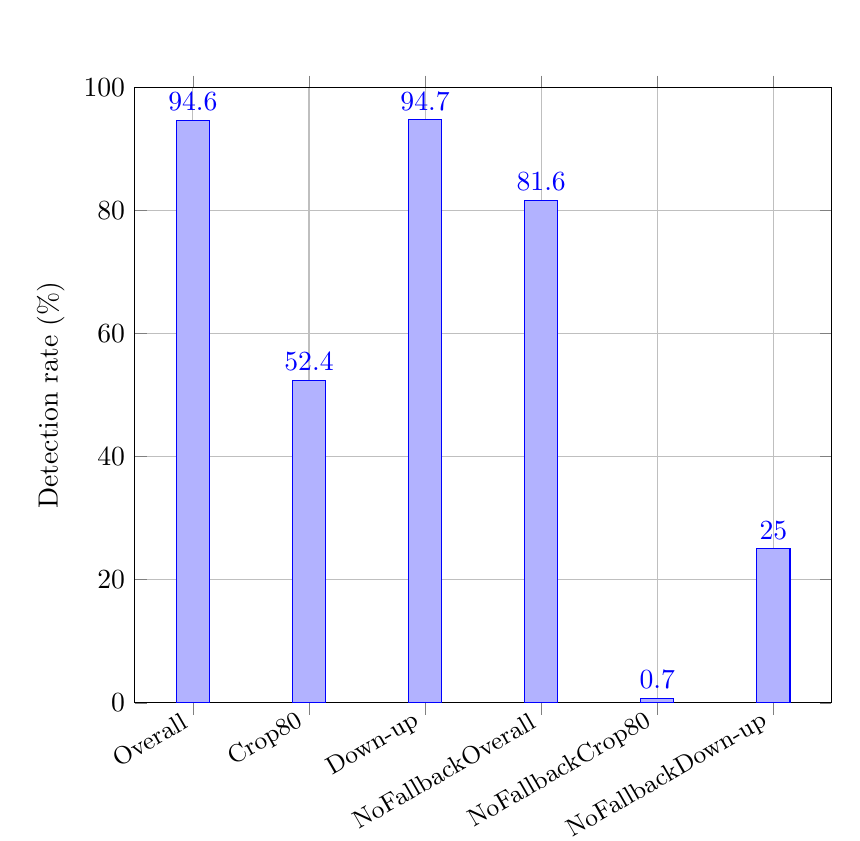
\begin{tikzpicture}
\begin{axis}[
width=0.86\textwidth,
height=3.7in,
ybar,
bar width=12pt,
ymin=0,
ymax=100,
ylabel={Detection rate (\%)},
symbolic x coords={Overall,Crop80,Down-up,NoFallbackOverall,NoFallbackCrop80,NoFallbackDown-up},
xtick=data,
x tick label style={rotate=30,anchor=east,font=\small},
nodes near coords,
nodes near coords align={vertical},
grid=major
]
\addplot coordinates {
(Overall,94.6)
(Crop80,52.4)
(Down-up,94.7)
(NoFallbackOverall,81.6)
(NoFallbackCrop80,0.7)
(NoFallbackDown-up,25.0)
};
\end{axis}
\end{tikzpicture}
\caption{Selected benchmark outcomes showing the value of global fallback detection}
\AltText{A bar chart comparing visible watermark detection results with and without global fallback. The chart highlights overall detection, severe crop performance, and down-up rescale performance, showing much stronger results when global fallback is enabled.}
\end{figure}

\section{Neural Watermarking Improvements During Development}
The neural branch improved substantially during the course of development. Earlier iterations suffered from several issues: direct frame replacement at reduced resolution degraded texture, chromatic shifts introduced visible color distortion, and naive majority-vote extraction often produced BER values close to random guessing under attack. The system was then refined through multiple implementation changes. The embedder was changed to compute a low-resolution residual and apply only the upsampled delta to the original frame. Color preservation modes were introduced, with a luminance-only option to minimize hue shifts. Edge feathering and Gaussian smoothing reduced halo artifacts. The extractor was upgraded to confidence-weighted voting over more frequent frame samples. The training setup was also extended to include resize down-up simulation and a GPU retraining workflow.

These changes improved the practical usefulness of the neural channel. In local application testing after retraining, representative attack sets showed neural BER values much better than the earlier 50\%--60\% range seen before retraining and extraction upgrades. The aggregate batch summary of approximately 29.99\% BER provides a useful overall reference point, while later interactive runs on selected attacks demonstrated even stronger behavior under some conditions. The neural channel is still not as deployment-ready as the visible channel, but it moved from speculative prototype status to a meaningful supporting component of the system.

\section{Traceability and Forensic Interpretation}
The traceability features are an important part of the system. Visible fingerprints can contain a direct user identifier or a short hash, while the DCT channel can carry a protected binary version of that information. This layered design matters in OTT piracy settings because a visible identifier offers quick human-readable evidence and an invisible payload adds hidden support when the visible overlay has been weakened.

\section{Manual Editing and Usability Outcomes}
The manual adjustment workflow improved the project's usability significantly. Automatic placement is useful, but real scenes still need exceptions. Keyframe interpolation makes repositioning practical, and frame-range suppression allows the visible watermark to be removed temporarily in sensitive shots such as close-up faces. These features make the system easier to use in realistic editing situations.

\section{Limitations and Interpretation of Results}
Although the results are strong in several respects, they should be interpreted carefully. The visible watermark benchmark is the most mature and convincing component of the evaluation. The DCT and neural channels are useful supporting elements, but they are less robust and more parameter-sensitive. Crop-heavy attacks remain difficult for all visible methods because geometry directly removes or displaces the rendered text. Neural watermarking remains a compromise between invisibility and robustness, and its observed BER, while improved, still indicates room for better training data, stronger attack curricula, or architecture redesign.

The system also depends on placement metadata for visible detection. This is a reasonable engineering choice, but it means the detector is not fully blind. For many operational scenarios, this is acceptable because the service generating the watermark can also store the metadata. From a pure watermarking-research perspective, however, blind detection would be a stricter requirement. The project therefore occupies a practical middle ground between theoretical purity and deployable engineering.

\section{Discussion}
Taken together, the results support a clear conclusion: adaptive visible watermarking with hybrid placement and fallback detection is the strongest part of the system, while the DCT and neural branches add useful forensic support without yet matching the visible channel in robustness. That balance is appropriate for a master's project because it shows both a strong core result and a realistic path for future improvement.

\clearpage
\chapter{CONCLUSION AND FUTURE WORK}
\section{Conclusion}
This project set out to build a video watermarking system that was not only technically interesting, but also practical to use and defend in a graduate report. The final system combines visible text overlays, adaptive placement based on frame content, temporal smoothing, optional optical flow, traceability support, invisible DCT payloads, and a neural watermarking branch. Just as importantly, it wraps those parts into a working application with generation, preview, manual editing, detection, and attack testing.

The clearest result is that the visible watermarking path performs well when it is paired with careful placement and fallback-aware detection. The reported benchmark of 94.6\% mean detection at threshold 0.40 across twenty-six HD clips and seventeen attacks is a strong outcome for a master's project. The ablation study strengthens that result by showing that the fallback search is not optional; it is one of the main reasons the detector remains useful under crop and resize attacks.

The invisible branches make the system broader and more realistic. The DCT path adds a hidden forensic payload with error-correction support. The neural path shows how a learned watermark can be integrated into the same application, while also making the quality-versus-robustness tradeoff very clear. After retraining and extractor improvements, the neural branch became much more useful than in its early form, even though it still does not match the reliability of the visible channel.

In the end, the project succeeds because it brings design, implementation, testing, and usability together in one coherent system. It shows how content-aware placement, saved metadata, layered watermark channels, and practical evaluation can work together in a way that is both academically credible and easy to demonstrate.

\section{Future Work}
Several future directions follow naturally from this project. The first is stronger content exclusion, especially face-aware placement or face-aware suppression, so that close-up human shots can be handled automatically rather than manually. The second is stronger invisible watermarking through better DCT coefficient strategies, better coding schemes, larger neural training sets, stronger attack simulation, and architectures designed for localized embedding rather than full-frame perturbation. The third is broader evaluation and deployment work, including richer perceptual metrics, stronger baseline comparisons, tighter integration with FastAPI and HLS workflows, and more complete forensic tooling for attribution and analyst review.

\clearpage
\begingroup
\singlespacing
\begin{thebibliography}{99}
\addcontentsline{toc}{chapter}{References}

\bibitem{lewis1995}
J. P. Lewis, ``Fast normalized cross-correlation,'' in \textit{Proceedings of Vision Interface}, 1995, pp. 120--123.

\bibitem{farneback2003}
G. Farneback, ``Two-frame motion estimation based on polynomial expansion,'' in \textit{Proceedings of the Scandinavian Conference on Image Analysis}, 2003, pp. 363--370.

\bibitem{deeplab}
L.-C. Chen, G. Papandreou, F. Schroff, and H. Adam, ``Rethinking atrous convolution for semantic image segmentation,'' arXiv preprint arXiv:1706.05587, 2017.

\bibitem{u2net}
Q. Qin, Z. Zhang, C. Huang, M. Dehghan, O. Zaiane, and M. Jagersand, ``U$^2$-Net: Going deeper with nested U-structure for salient object detection,'' \textit{Pattern Recognition}, vol. 106, 2020.

\bibitem{raft}
Z. Teed and J. Deng, ``RAFT: Recurrent all-pairs field transforms for optical flow,'' in \textit{Proceedings of the European Conference on Computer Vision}, 2020.

\bibitem{resnet}
K. He, X. Zhang, S. Ren, and J. Sun, ``Deep residual learning for image recognition,'' in \textit{Proceedings of the IEEE Conference on Computer Vision and Pattern Recognition}, 2016, pp. 770--778.

\bibitem{dctwm}
B. Chen and G. W. Wornell, ``Quantization index modulation: A class of provably good methods for digital watermarking and information embedding,'' \textit{IEEE Transactions on Information Theory}, vol. 47, no. 4, pp. 1423--1443, 2001.

\bibitem{reedsolomon}
I. S. Reed and G. Solomon, ``Polynomial codes over certain finite fields,'' \textit{Journal of the Society for Industrial and Applied Mathematics}, vol. 8, no. 2, pp. 300--304, 1960.

\bibitem{aesgcm}
M. Dworkin, ``Recommendation for block cipher modes of operation: Galois/Counter Mode (GCM) and GMAC,'' NIST Special Publication 800-38D, 2007.

\bibitem{ottpiracy}
M. C. Stamm, M. Wu, and K. J. R. Liu, ``Information forensics: An overview of the first decade,'' \textit{IEEE Access}, vol. 1, pp. 167--200, 2013.

\bibitem{videoseal}
Meta Research, ``VideoSeal: Open neural video watermarking,'' arXiv preprint arXiv:2402.11668, 2024.

\bibitem{itov}
G. Ye, J. Gao, Y. Wang, L. Song, and X. Wei, ``ItoV: Efficiently adapting deep learning-based image watermarking to video watermarking,'' arXiv preprint arXiv:2305.02781, 2023.

\bibitem{saliency}
A. Garcia-Diaz, X. R. Fdez-Vidal, X. M. Pardo, and R. Dosil, ``Decorrelation and distinctiveness provide with human-like saliency,'' in \textit{Proceedings of the International Conference on Advanced Concepts for Intelligent Vision Systems}, 2009.

\bibitem{opencv}
G. Bradski, ``The OpenCV Library,'' \textit{Dr. Dobb's Journal of Software Tools}, 2000.

\bibitem{pytorch}
A. Paszke et al., ``PyTorch: An imperative style, high-performance deep learning library,'' in \textit{Advances in Neural Information Processing Systems}, 2019.

\bibitem{streamlit}
Streamlit Inc., ``Streamlit documentation,'' 2024. [Online]. Available: \url{https://streamlit.io}

\bibitem{ffmpeg}
FFmpeg Developers, ``FFmpeg documentation,'' 2024. [Online]. Available: \url{https://ffmpeg.org}

\bibitem{davis}
F. Perazzi, J. Pont-Tuset, B. McWilliams, L. Van Gool, M. Gross, and A. Sorkine-Hornung, ``A benchmark dataset and evaluation methodology for video object segmentation,'' in \textit{Proceedings of the IEEE Conference on Computer Vision and Pattern Recognition}, 2016.

\end{thebibliography}
\endgroup

\end{document}
